\documentclass[11pt, aspectratio=169]{beamer}
%\documentclass{beamer}
\setbeamertemplate{navigation symbols}{}
\usetheme{Boadilla}
\usecolortheme{beaver}
\usepackage{caption}


\usepackage{tikz} 
\usepackage{adjustbox}

\usepackage{graphicx}
\usepackage{subcaption}
\usepackage{algorithm}
\usepackage{algpseudocode}
%\usepackage[noend]{algorithmic}
\usepackage{amsmath}
\usefonttheme{professionalfonts}
\usepackage{helvet}
\renewcommand{\familydefault}{\sfdefault}
%\renewcommand{\figurename}{Gambar}
\usepackage{hanging}
\usepackage{lipsum}
\usepackage{listings}
\newcommand\blfootnote[1]{%
  \begingroup
  \renewcommand\thefootnote{}\footnote{#1}%
  \addtocounter{footnote}{-1}%
  \endgroup
}
\setbeamertemplate{caption}{\insertcaption}

\setbeamertemplate{footnote}{\tiny \hangpara{1em}{1}\makebox[1em][l]{\insertfootnotemark}\footnotesize\insertfootnotetext\par}
\hyphenation{}

\usepackage{ragged2e}
\renewcommand\thempfootnote{\arabic{mpfootnote}}



%=======================================================
%KETERANGAN FRAME
\title[Progressive Edge-Growth (PEG) Algorithm]{Introduction to Progressive Edge-Growth (PEG) Algorithm for LDPC Codes}
%\subtitle{Avoiding Common Mistakes}
\author[Afa]{ 
%	\vspace{-0.1in}
%
\includegraphics[height=0.35in]{gambarafa/logoSOFTT}
%\hspace{0.05in}

\includegraphics[height=0.35in]{gambarafa/adwitech}
\hspace{0.05in}
%
\includegraphics[height=0.35in]{gambarafa/telu.jpg}
\\ \quad \\Citra Yasin Akbar Fadhlika}
\institute[AdWiTech, Telkom Univ.] { The Center for Advanced Wireless Technologies (AdWiTech), Telkom University,\\
Jl. Telekomunikasi No. 1, Terusan Buah Batu, Bandung, 40257 Indonesia.\\
E-mail: \{\textit{citrayaf@student.\}telkomuniversity.ac.id}
%\blfootnote{\tiny{This research is supported in part by the World Class Research Grant for T3LESDM-Net, 20192021.}}
}

\date[November $19^{th}, 2019$]{\small ZEMI\\
Bandung, Indonesia }


%			LET'S START YEYEYEYYEYE
%========================================================
% Let's get started the document
\begin{document}
\justifying

\begin{frame}
  \titlepage
\end{frame}
\begin{frame}{Outline}
  \tableofcontents
  % You might wish to add the option [pausesections]
\end{frame}
%-----------------------------------------------------------------------


%=======================================================
%=======================================================
\section{Motivation and Problem}
%--------------------------------------
\begin{frame}{Motivation and Problem}
%--------------------------------------
%\begin{figure}
%\centering
%
\includegraphics[scale=0.35]{gambarafa/migrasi}
%\caption{Indonesia Digital Television Standard Migration.}
%\label{downlink} 
%\end{figure}
%\vspace{-10pt}
\begin{itemize}
\justifying
\item Perancangan matriks \textit{parity check} $H$ LDPC \textit{codes} tidak bisa dilakukan secara \textit{random}, oleh karena itu teknik perancangan matriks $H$ LDPC \textit{codes} harus menghasilkan \textit{girth} besar.
\item Nilai \textit{girth} kecil akan memperburuk kinerja dari \textit{iterative decoding} LDPC codes.\footnote[1]{\tiny M. Sipser and D. A. Spielman, "Expander codes," in IEEE Transactions on Information Theory, vol. 42, no. 6, pp. 1710-1722, Nov. 1996.}
\end{itemize}
\end{frame}

%=======================================================
%=======================================================
\section{Basic Theory}

%--------------------------


%--------------------------
\begin{frame}{Low Density Parity Check (LDPC) Codes}
	\framesubtitle{}
	\begin{itemize}
		\item LDPC \textit{codes} terbentuk oleh sebuah matriks yang sebagian besar elemennya bernilai $"0"$ dan hanya beberapa yang bernilai $"1"$.\footnote[1]{\tiny R. Gallager, "Low-density parity-check codes," in IRE Transactions on Information Theory, vol. 8, no. 1, pp. 21-28, January 1962.} \\
		\item LDPC \textit{codes} memiliki kinerja yang baik pada panjang blok $n$ mendekati tak hingga dan cenderung memiliki kinerja yang lebih buruk pada $n$ yang terbatas.\footnote[2]{\tiny T. J. Richardson and R. L. Urbanke, "The capacity of low-density parity-check codes under message-passing decoding," in IEEE Transactions on Information Theory, vol. 47, no. 2, pp. 599-618, Feb 2001.
		} \\
		
		\item Matriks \textit{parity check} $H$\\
		\begin{itemize}
			\item[$\checkmark$] Panjang blok $n$\\
			\item[$\checkmark$] \textit{Variable node degree} $d_v$\\
			\item[$\checkmark$] \textit{Check node degree} $d_c$\\    		
		\end{itemize}
	
	\end{itemize}
	%\begin{figure}[]
	%	\begin{picture}(0,0)
	%	\tiny {\centering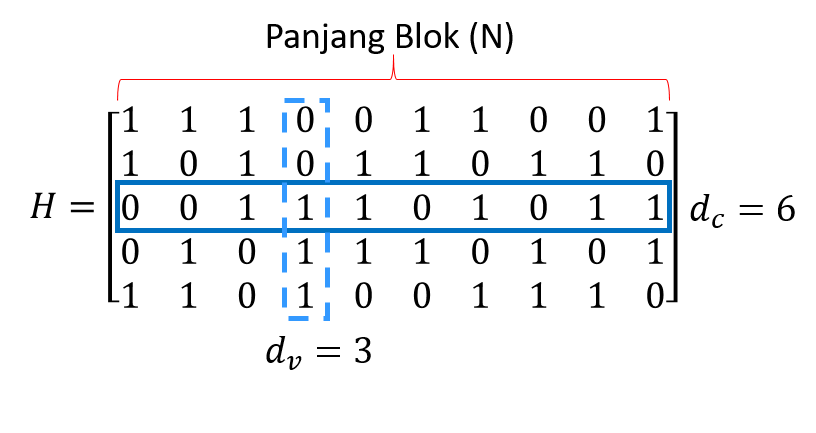
\includegraphics[scale=.6]{pict/ldpc.png}
	%		\caption{Transmitter and receiver diagram block of QC-LDPC codes wireless communication systems.}}
	%	\end{picture}
	%	\label{fig:LDPC}
	%\end{figure}
	\begin{figure}
		\begin{picture}(0,0)
		\put(-15,-30){
			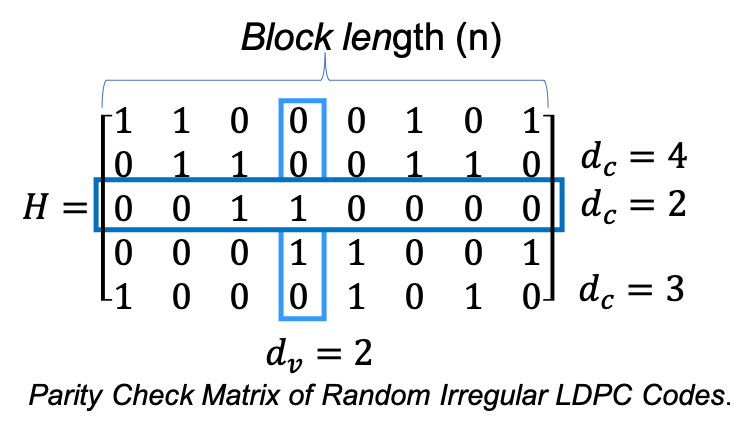
\includegraphics[scale=.5]{gambarafa/matrixirre.png}
			
		}
		
		\end{picture}
		%	\caption{\footnotesize Parity Check Matrix of Regular (3,6) LDPC codes.}
	\end{figure}

	
	%	\footnotetext[1]{\cite{koding1}}
	%	\footnotetext[2]{\cite{ldpc6}}
	%	\footnotetext[3]{\cite{ldpc5}}
\end{frame}
%=======================================================
%=======================================================
\begin{frame}{Tanner Graph}
%--------------------------
\vspace{-1cm}
\begin{figure}
\centering 
\includegraphics[scale=0.6]{gambarafa/TannerH}
\centering 
\label{sistemmodelMQCLDPC} %~\ref{kucing}
\end{figure}

\begin{itemize}
%\item SIMPLE : Small block size less than 2000
\item Matriks \textit{parity check} LDPC \textit{codes} $H$ dapat direpresentasikan menggunakan Tanner \textit{graph} dengan dua set \textit{node}.\footnote[1]{\tiny R. Tanner, "A recursive approach to low complexity codes," in IEEE Transactions on Information Theory, vol. 27, no. 5, pp. 533-547, September 1981.
} 
\item Garis (\textit{edge}) antara \textit{variable nodes} dengan \textit{check nodes} terhubung apabila 
\begin{equation}
 H_{i,j}=1,
\end{equation}
dengan $i$ adalah \textit{variable node} ke-$i$ dan $j$ adalah \textit{check node} ke-$j$.


%\item The systems use narrowband system with single carrier transmission.
%\item Channels are Additive White Gaussian Noise (AWGN) and frequency-flat Rayleigh fading.
%\item Perfect channel synchronization and estimation.
%\begin{itemize}
%\item Matrix Generator $G$ in encoder.
%\item Parity Check Matrix $H$ in decoder. 
%\end{itemize}
%\vspace{-0.35cm}
%\begin{eqnarray}
%\mathbf{G}\cdot \mathbf{H}^T&=&0.
%\end{eqnarray}
\end{itemize}

\vspace{-20pt}
%\begin{figure}
%\centering 
%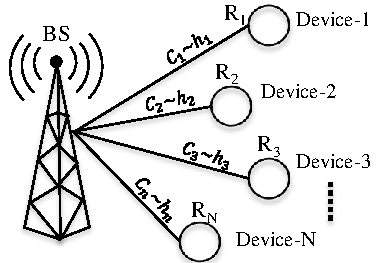
\includegraphics[scale=0.85]{pics/downlink2.pdf}
%\caption{Configuration of downlink IoT wireless communication systems.}
%\label{massiveiot} %~\ref{kucing}
%\end{figure}

\end{frame}
%%--------------------------
%\begin{frame}{Basic Theory}
%%--------------------------
%\begin{itemize}
%\item Low-Density Parity-Check (LDPC) codes were introduced by Gallager in his PhD dissertation in the 1960s.
%\item LDPC codes are binary linear block codes with a sparse parity-check matrix $\mathbf{H}$ that has most of its elements as 0s.
%%\item Low latency channel coding and low complexity.
%\end{itemize}
%\begin{columns}
%\column{.45\textwidth}
%\begin{eqnarray}
%\mathbf{G}&=&[I_k\; P],\\
%\mathbf{H}&=&[-P^T\; I_{n-k}],\\
%\mathbf{G}\cdot \mathbf{H}^T&=&0.
%\end{eqnarray}
%\column{.55\textwidth}
%\begin{figure}
%\centering %taro di tengah
%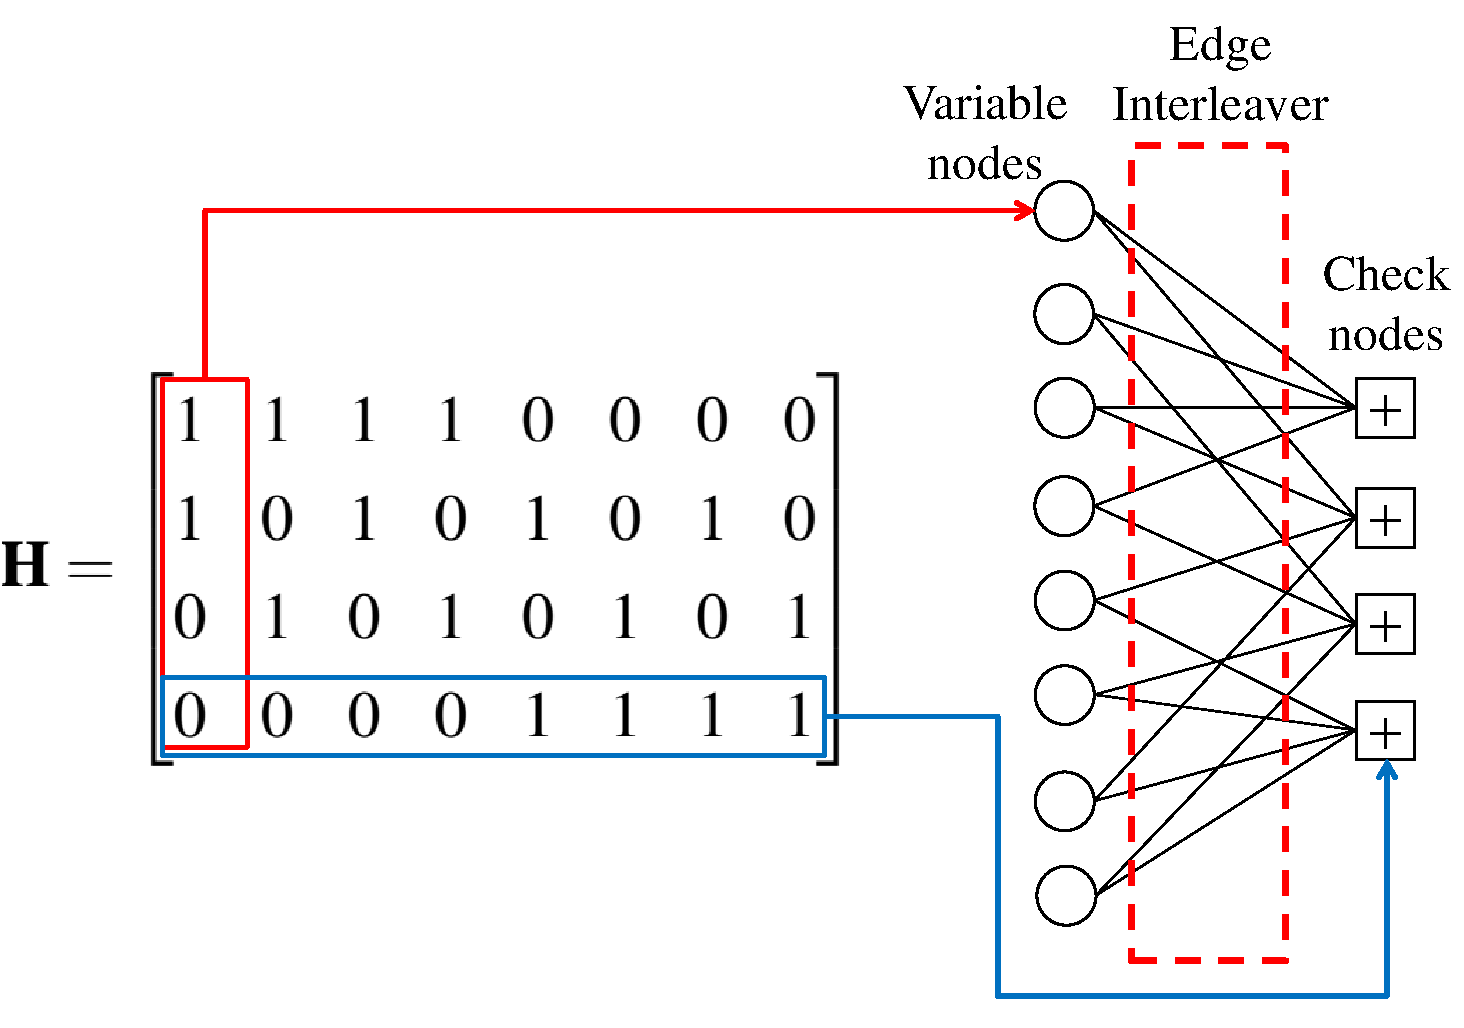
\includegraphics[scale=0.25]{pics/bipartitH1.pdf}
%\caption{Bipartite graph of parity check matrix $\mathbf{H}$.}
%\label{bipartitH} 
%\end{figure}
%\end{columns}
%\end{frame}
\begin{frame}{\textit{Girth}}
%--------------------------
\begin{figure}
	\centering 
	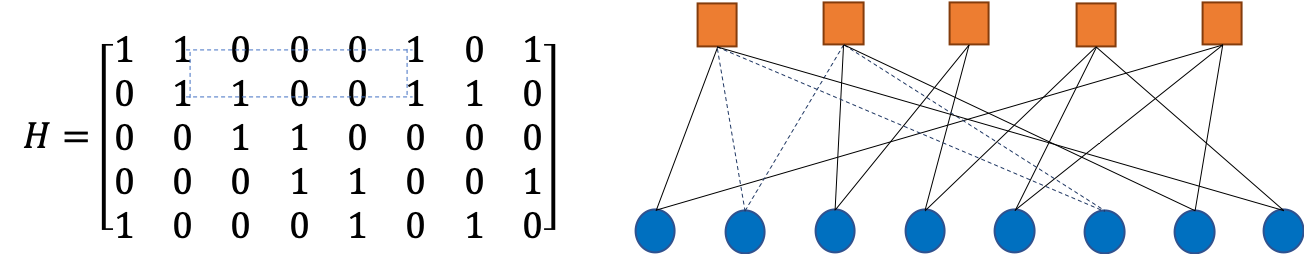
\includegraphics[scale=0.6]{gambarafa/GirthH}
	\centering 
\end{figure}
\begin{itemize}
	\item \textit{Girth} adalah panjang siklus terpendek dalam sebuah Tanner \textit{graph} yang menjadi hal penting dalam menentukan kinerja LDPC \textit{codes}.\footnote[1]{\tiny J. Fan and Y. Xiao, "A Method of Counting the Number of Cycles in LDPC Codes," 2006 8th international Conference on Signal Processing, Beijing, 2006, pp.}  
	\item \textit{Girth} lokal pun terbentuk dari siklus per \textit{node} pada sebuah Tanner \textit{graph} LDPC \textit{codes}.  
	\item Terjadinya \textit{girth} kecil akan memberikan efek buruk pada LDPC codes, karena mengurangi kinerja dari \textit{extrinsic information} dalam proses \textit{iterative decoding}.\footnote[2]{\tiny M. Sipser and D. A. Spielman, "Expander codes," in IEEE Transactions on Information Theory, vol. 42, no. 6, pp. 1710-1722, Nov. 1996.}  
	
\end{itemize}

.

\end{frame}


%--------------------------
\begin{frame}{Progresive Edge-Growth (PEG) Algorithm (1/4)\footnote[1]{\tiny Xiao-Yu Hu, E. Eleftheriou and D. -. Arnold, "Progressive edge-growth Tanner graphs," GLOBECOM'01. IEEE Global Telecommunications Conference (Cat. No.01CH37270), San Antonio, TX, 2001, pp. 995-1001 vol.2.}}
%--------------------------
\begin{itemize}
	\item PEG adalah salah satu metode untuk membuat LDPC \textit{codes} berdasarkan dari Tanner \textit{graph} dengan memperhatikan penyebaran \textit{edge} yang terhubung pada setiap \textit{node} untuk menghasilkan \textit{girth} besar.
	\item Pembuatan LDPC codes dengan menggunakan PEG dapat dibuat berdasarkan jumlah \textit{variable nodes} atau \textit{block length} $n$, check node $m$, \textit{variable node degree} (VND), dan \textit{check node degree} (CND).
	\item PEG melakukan penyebaran \textit{edge} menggunakan graf pohon dengan memperhatikan \textit{degree} setiap \textit{node} yang telah ditentukan dan setiap \textit{node}-nya hanya dapat muncul sekali.
	\item Kedalaman dari graf pohon akan disimbolkan dengan $l$. $l$ akan mempengaruhi lokal \textit{girth} yang terbentuk.
\end{itemize}

\end{frame}

%=======================================================
\begin{frame}{Progresive Edge-Growth (PEG) Algorithm (2/4)}
	%--------------------------
	Secara sederhana proses pembuatan LDPC \textit{codes} menggunakan algoritma PEG adalah sebagai  berikut:
	\begin{enumerate}
		\item Tempatkan elemen 1 mulai dari kolom ke-1 sampai ke-$n$, penempatan ini memperhatikan baris atau \textit{check node} dengan \textit{degree} terkecil.
		\item Menyebarkan \textit{edge} ke node yang belum terhubung dengan memperhatikan \textit{degree} dari \textit{check node}.
	\end{enumerate}
	\textit{Cycle} dari LDPC \textit{codes} yang terbentuk menggunakan PEG dapat dipastikan akan memenuhi 
	\begin{equation}
		2(l+2).
	\end{equation}


	
	
	%\blfootnote{\tiny{ETSI, Digital Video Broadcasting (DVB); Frame Structure Channel Coding and Modulation for a Second Generation Digital Terrestrial Television Broadcasting System (DVB-T2), 1st ed., ETSI, July 2015.}}
	%\begin{figure}
	%\centering
	%\hspace{-0.2in} 
	%\begin{tabular}{cl}
	%$\mathbf{H}=$ & \begin{tabular}[c]{@{}l@{}}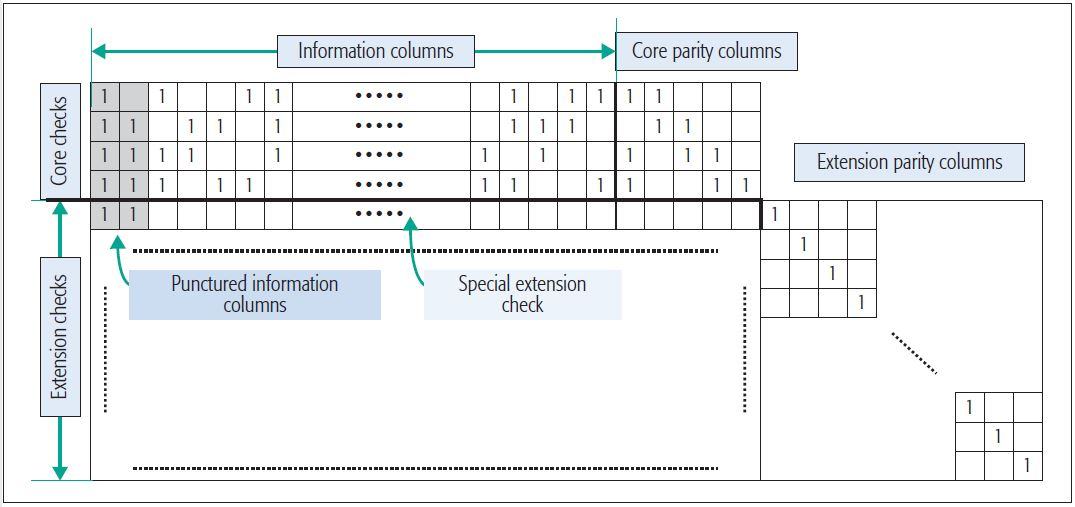
\includegraphics[scale=0.38]{pics/matriks5g}\end{tabular}
	%\end{tabular}
	%\caption{Sketch of base parity check structure for the 5G-NR LDPC codes \footnote{\tiny{T. Richardson and S. Kudekar, “Design of low-density parity check codes for 5G new radio,” IEEE Communications Magazine, vol. 56, no. 3, pp. 28–34, March 2018.}}.}
	%\label{5gsketch}
	%\end{figure}
	%\end{columns}
\end{frame}
%=======================================================
\begin{frame}{Progresive Edge-Growth (PEG) Algorithm (3/4)\footnote[1]{\tiny Xiao-Yu Hu, E. Eleftheriou and D. M. Arnold, "Regular and irregular progressive edge-growth tanner graphs," in IEEE Transactions on Information Theory, vol. 51, no. 1, pp. 386-398, Jan. 2005.
	}}
	%--------------------------
%	Dalam perancangan LDPC \textit{codes} menggunakan algoritma PEG dengan nilai $d_v$, $d_c$, dan $m$ yang telah ditentukan, dapat diketahui batas dari nilai \textit{girth} melalui persamaan
\vspace{-0.2cm}
	Batas nilai \textit{girth} $(g)$ pada LDPC \textit{codes} yang dirancang menggunakan algoritma PEG dapat diketahui melalui persamaan 
	\begin{equation}
	t=\frac{\log\left ( md_c^{max}- \frac{md_c^{max}}{d_v^{max}} - m +1 \right )}{\log\left [ \left ( d_v^{max} -1  \right ) \left ( d_c^{max} -1  \right ) \right ]}-1,
	\label{eq:t}
	\end{equation}
	\begin{equation}
		g \geq 2 \left (\left \lfloor t \right \rfloor +2 \right ),
		\label{eq:g}
	\end{equation}
	dengan nilai $d_v$, $d_c$, dan $m$ yang telah ditentukan. Dari persamaan (\ref{eq:t}) dan (\ref{eq:g}) maka
	\begin{equation}
	\frac{d_v^{max}\left [  \left ( d_v^{max}-1 \right )^{t+1} \left ( d_c^{max}-1 \right )^{t+1} -1\right ]}{\left ( d_v^{max}-1 \right ) \left ( d_c^{max}-1 \right )-1}<m,
	\end{equation}
	sehingga dapat diketahui batas minimal jumlah \textit{check node} agar \textit{girth} yang ingin dihindari dapat terpenuhi.
\end{frame}



\begin{frame}{Progresive Edge-Growth (PEG) Algorithm (4/4)}
	%--------------------------
	PEG memiliki dua metode dalam proses pembuatan LDPC \textit{codes} dengan cara:
	\begin{enumerate}
		\item Secara acak memilih \textit{check nodes} terkecil yang ditemukan.
		\item Selalu memilih \textit{check nodes} terkecil yang ditemukan sesuai dengan urutannya $c_1, c_2, c_3, \cdots, c_{m}$, dengan $m$ adalah jumlah baris.
	\end{enumerate}
	Hal ini mengakibatkan LDPC \textit{codes} akan memiliki matriks \textit{parity check} berbeda-beda, apabila menggunakan algoritma PEG. Pada awalnya PEG menggunakan metode pertama\footnote[1]{\tiny Xiao-Yu Hu, E. Eleftheriou and D. M. Arnold, "Regular and irregular progressive edge-growth tanner graphs," in IEEE Transactions on Information Theory, vol. 51, no. 1, pp. 386-398, Jan. 2005.}, sedangkan pada penelitian ini mengusulkan dengan menggunakan metode kedua.

\end{frame}


\section{The Proposed PEG Algorithm for LDPC Codes}
%--------------------------
\begin{frame}{The Proposed PEG Algorithm for LDPC Codes}
%--------------------------
\begin{itemize}
\item Algoritma PEG yang diusulkan menggunakan metode kedua dan ditambahkan sebuah algoritma untuk menghindari pembentukkan LDPC \textit{codes} dengan \textit{girth}-4.
\item Penggunaan PEG dalam pembuatan matriks \textit{parity check} LDPC \textit{codes} memungkinkan untuk membuat matriks \textit{parity check} LDPC \textit{codes} sesuai dengan keinginan.
\item Nilai panjang blok $n$, baris $m$, dan set dari VND~$D_v=\{ d_{v_1}, d_{v_2}, d_{v_3}, \cdots ,d_{v_n} \}$ dapat ditentukan, dengan $d_v$ adalah VND.
\item Proses penempatan elemen 1 dimulai dari kolom 1 sampai $n$ dan dari baris 1 ke $m$ yang prosesnya berjalan dari kiri ke kanan dan dari atas ke bawah.
%\item Algoritma anti \textit{girth}-4 ini ditambahkan pada iterasi kedua dalam penempatan elemen satu di setiap kolom. Langkah-langkah pengecekan:
%\begin{enumerate}
%	\item Melukakan pencarian elemen 1 pada kolom yang sama dengan posisi yang akan kita tambahkan elemen 1, apabila ditemukan simpan baris dari elemen 1 tersebut.
%	\item 
%\end{enumerate}
\end{itemize}
\blfootnote{\tiny{F. A. Newagy and S. H. Elramly, “Novel Technique for Scaling Down LDPC Code Lengths in DVB-T2 Standard,” in 2012 International Conference on Telecommunications and Multimedia (TEMU), July 2012, pp. 180–184.}}
\end{frame}

%--------------------------
\begin{frame}{The Proposed Anti Girth-4 Algorithm (1/5)}
%--------------------------

\centering 
\begin{itemize}
\item Algoritma anti \textit{girth}-4 ini ditambahkan pada iterasi kedua dalam penempatan elemen satu di setiap kolom. Langkah-langkah perancangan matriks dan pengecekannya sebagai berikut:
\begin{figure}
				\centering 
			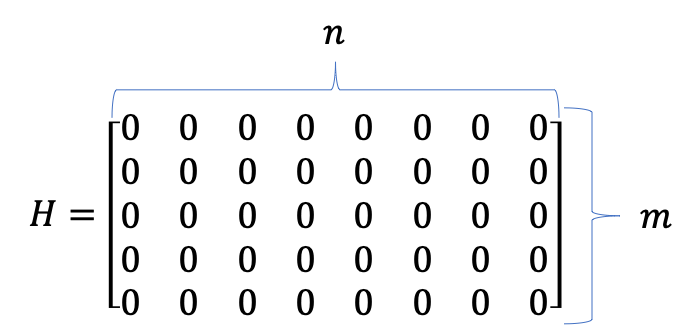
\includegraphics[scale=0.5]{gambarafa/step1}
			\centering 
		\end{figure}
\begin{itemize}
	\item[1.] Buat matriks nol dengan dimensi $m\times n$, dengan $n$ adalah jumlah variable \textit{nodes} dan $m$ adalah jumlah \textit{check nodes} yang telah ditentukan.
\end{itemize}
%\begin{enumerate}
%	\begin{figure}
%			\centering 
%		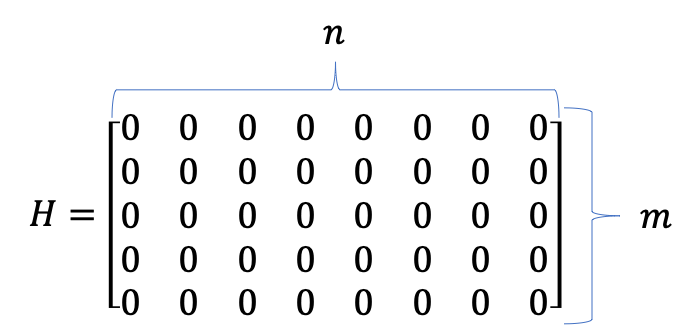
\includegraphics[scale=0.5]{gambarafa/step1}
%		\centering 
%	\end{figure}
%	\item Melukakan pencarian elemen 1 pada kolom yang sama dengan posisi yang akan kita tambahkan elemen 1, apabila ditemukan simpan baris dari elemen 1 tersebut.
%	\item Kemudian melakukan pengecekan kembali pada satu baris yang sama dengan posisi yang akan kita tambahkan elemen 1, apabila ditemukan simpan kolom dari elemen satu tersebut.
%	\item Apabila pada langkah pertama dan kedua tidak ditemukan elemen satu maka posisi yang akan kita tambahkan elemen 1 akan aman dari \textit{girth}-4, jika ditemukan maka lanjut ke langkah berikutnya.
%	\item Melakukan pengecekan pada elemen matriks dengan kolom dan baris yang tersimpan, apabila bernilai 1 maka posisi tersebut tidak boleh bernilai 1 jika tidak maka posisi tersebut dapat bernilai 1.
%\end{enumerate}

\end{itemize}





%\begin{table}[tb]
%		\caption{addresses of parity bit accumulators for $N_{LDPC}=16200$ with code rate $R=\frac{1}{2}$.}
%	\label{table:accu}
%	\begin{tabular}{|l|l|l|lllll}
%		\hline
%		\multicolumn{1}{|c|}{20} & \multicolumn{1}{c|}{712}  & \multicolumn{1}{c|}{2386} & \multicolumn{1}{c|}{6354} & \multicolumn{1}{c|}{4061} & \multicolumn{1}{c|}{1062} & \multicolumn{1}{c|}{5045} & \multicolumn{1}{c|}{5158} \\ \hline
%		\multicolumn{1}{|c|}{21} & \multicolumn{1}{c|}{2543} & \multicolumn{1}{c|}{5748} & \multicolumn{1}{c|}{4822} & \multicolumn{1}{c|}{2348} & \multicolumn{1}{c|}{3089} & \multicolumn{1}{c|}{6328} & \multicolumn{1}{c|}{5876} \\ \hline
%		\multicolumn{1}{|c|}{22} & \multicolumn{1}{c|}{926}  & \multicolumn{1}{c|}{5701} & \multicolumn{1}{c|}{269}  & \multicolumn{1}{c|}{3693} & \multicolumn{1}{c|}{2438} & \multicolumn{1}{c|}{3190} & \multicolumn{1}{c|}{3507} \\ \hline
%		\multicolumn{1}{|c|}{23} & \multicolumn{1}{c|}{2802} & \multicolumn{1}{c|}{4520} & \multicolumn{1}{c|}{3577} & \multicolumn{1}{c|}{5324} & \multicolumn{1}{c|}{1091} & \multicolumn{1}{c|}{4667} & \multicolumn{1}{c|}{4449} \\ \hline
%		\multicolumn{1}{|c|}{24} & \multicolumn{1}{c|}{5140} & \multicolumn{1}{c|}{2003} & \multicolumn{1}{c|}{1263} & \multicolumn{1}{c|}{4742} & \multicolumn{1}{c|}{6497} & \multicolumn{1}{c|}{1185} & \multicolumn{1}{c|}{6202} \\ \hline
%		0                        & 4046                      & 6934                      &                           &                           &                           &                           &                           \\ \cline{1-3}
%		1                        & 2855                      & 66                        &                           &                           &                           &                           &                           \\ \cline{1-3}
%		2                        & 6694                      & 212                       &                           &                           &                           &                           &                           \\ \cline{1-3}
%		3                        & 3439                      & 1158                      &                           &                           &                           &                           &                           \\ \cline{1-3}
%		4                        & 3850                      & 4422                      &                           &                           &                           &                           &                           \\ \cline{1-3}
%		5                        & 5924                      & 290                       &                           &                           &                           &                           &                           \\ \cline{1-3}
%		6                        & 1467                      & 4049                      &                           &                           &                           &                           &                           \\ \cline{1-3}
%		7                        & 7820                      & 2242                      &                           &                           &                           &                           &                           \\ \cline{1-3}
%		8                        & 4606                      & 3080                      &                           &                           &                           &                           &                           \\ \cline{1-3}
%		9                        & 4633                      & 7877                      &                           &                           &                           &                           &                           \\ \cline{1-3}
%		10                       & 3884                      & 6868                      &                           &                           &                           &                           &                           \\ \cline{1-3}
%		11                       & 8935                      & 4996                      &                           &                           &                           &                           &                           \\ \cline{1-3}
%		12                       & 3028                      & 764                       &                           &                           &                           &                           &                           \\ \cline{1-3}
%		13                       & 5988                      & 1057                      &                           &                           &                           &                           &                           \\ \cline{1-3}
%		14                       & 7411                      & 3450                      &                           &                           &                           &                           &                           \\ \cline{1-3}
%	\end{tabular}
%\end{table}

\end{frame}


\begin{frame}{The Proposed Anti Girth-4 Algorithm (2/5)}
	%--------------------------
	
	\centering 
		\begin{figure}
			\centering 
			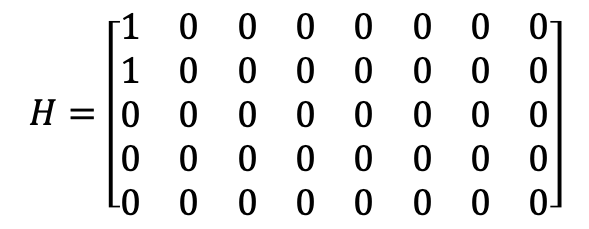
\includegraphics[scale=0.5]{gambarafa/step2}
			\centering 
		\end{figure}
		\begin{itemize}
			\item[2.] Elemen 1 pertama ditempatkan sesuai dengan algoritma pertama dari proses PEG. Elemen 1 kedua dan seterusnya sebanyak $d_v(n)$ ditempatkan menggunakan kombinasi algoritma PEG dengan \textit{Anti Girth}-4.
		\end{itemize}
	\centering 
	\begin{figure}
		\centering 
		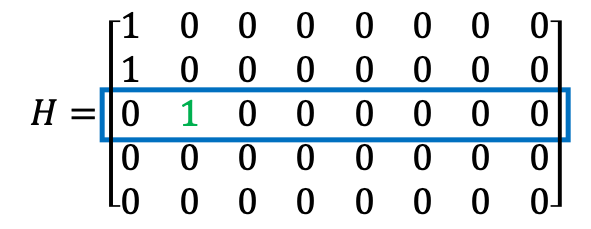
\includegraphics[scale=0.5]{gambarafa/step3}
		\centering 
	\end{figure}
	\begin{itemize}
		\item[3.] Elemen 1 ditempatkan pada \textit{check node} urutan pertama dengan nilai CND terendah.
	\end{itemize}
		%\begin{enumerate}
		%	\begin{figure}
		%			\centering 
		%		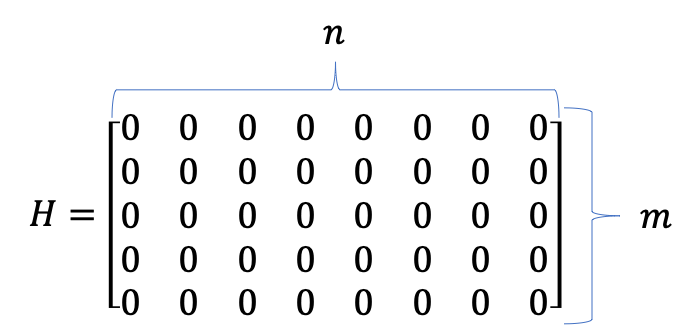
\includegraphics[scale=0.5]{gambarafa/step1}
		%		\centering 
		%	\end{figure}
		%	\item Melukakan pencarian elemen 1 pada kolom yang sama dengan posisi yang akan kita tambahkan elemen 1, apabila ditemukan simpan baris dari elemen 1 tersebut.
		%	\item Kemudian melakukan pengecekan kembali pada satu baris yang sama dengan posisi yang akan kita tambahkan elemen 1, apabila ditemukan simpan kolom dari elemen satu tersebut.
		%	\item Apabila pada langkah pertama dan kedua tidak ditemukan elemen satu maka posisi yang akan kita tambahkan elemen 1 akan aman dari \textit{girth}-4, jika ditemukan maka lanjut ke langkah berikutnya.
		%	\item Melakukan pengecekan pada elemen matriks dengan kolom dan baris yang tersimpan, apabila bernilai 1 maka posisi tersebut tidak boleh bernilai 1 jika tidak maka posisi tersebut dapat bernilai 1.
		%\end{enumerate}
		

	
	
\end{frame}
%=======================================================
\begin{frame}{The Proposed Anti Girth-4 Algorithm (3/5)}
	%--------------------------
	
	\centering 
	\begin{figure}
		\centering 
		
\includegraphics[scale=0.75]{gambarafa/step4}
		\centering 
	\end{figure}
	\begin{itemize}
		\item[4.] Simbol $x$ adalah calon letak elemen 1, $x$ dipilih berdasarkan baris yang memiliki nilai CND terendah. Kemudian langkah berikutnya menggunakan algoritma \textit{Anti Girth}-4, melakukan pengeceken ke kiri apabila tidak ada elemen satu maka letak tersebut akan menjadi elemen 1.
	\end{itemize}
%	\centering 
%	\begin{figure}
%		\centering 
%		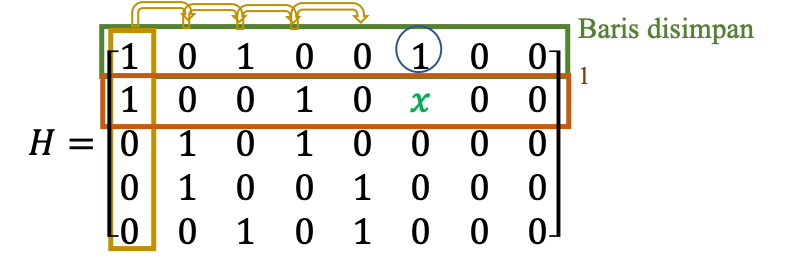
\includegraphics[scale=0.5]{gambarafa/step5}
%		\centering 
%	\end{figure}
%	\begin{itemize}
%		\item[5.] Elemen 1 ditempatkan pada \textit{check node} urutan pertama dengan nilai CND terendah.
%	\end{itemize}
	%\begin{enumerate}
	%	\begin{figure}
	%			\centering 
	%		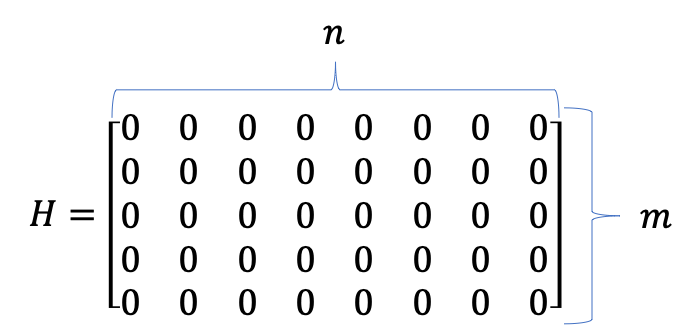
\includegraphics[scale=0.5]{gambarafa/step1}
	%		\centering 
	%	\end{figure}
	%	\item Melukakan pencarian elemen 1 pada kolom yang sama dengan posisi yang akan kita tambahkan elemen 1, apabila ditemukan simpan baris dari elemen 1 tersebut.
	%	\item Kemudian melakukan pengecekan kembali pada satu baris yang sama dengan posisi yang akan kita tambahkan elemen 1, apabila ditemukan simpan kolom dari elemen satu tersebut.
	%	\item Apabila pada langkah pertama dan kedua tidak ditemukan elemen satu maka posisi yang akan kita tambahkan elemen 1 akan aman dari \textit{girth}-4, jika ditemukan maka lanjut ke langkah berikutnya.
	%	\item Melakukan pengecekan pada elemen matriks dengan kolom dan baris yang tersimpan, apabila bernilai 1 maka posisi tersebut tidak boleh bernilai 1 jika tidak maka posisi tersebut dapat bernilai 1.
	%\end{enumerate}
	
	
	
	
\end{frame}

	%--------------------------
\begin{frame}{The Proposed Anti Girth-4 Algorithm (4/5)}
	
	\centering 
	\begin{figure}
		\centering 
		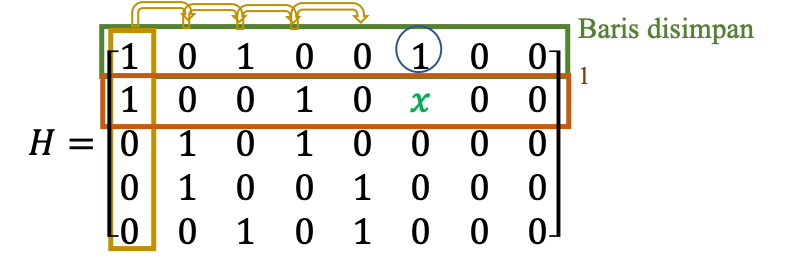
\includegraphics[scale=0.65]{gambarafa/step5}
		\centering 
	\end{figure}
	\begin{itemize}
		\item[5.] Algoritma \textit{Anti Girth}-4 dimulai dari iterasi ke-1, baris dari elemen 1 sebelumnya disimpan yang nantinya akan digunakan pada pengecekan akhir. Kemudian melakukan pengecekan dari kiri ke kanan apabila ditemukan elemen 1, maka akan berlanjut ke iterasi berikutnya. Apabila tidak ditemukan elemen 1 pada kolom tersebut, maka $x$ akan menjadi elemen 1. Pengecekan akan dilakukan sampai kolom sebelum kolom dari $x$.
	\end{itemize}





\end{frame}

\begin{frame}{The Proposed Anti Girth-4 Algorithm (5/5)}
	
	\centering 
	\begin{figure}
		\centering 
		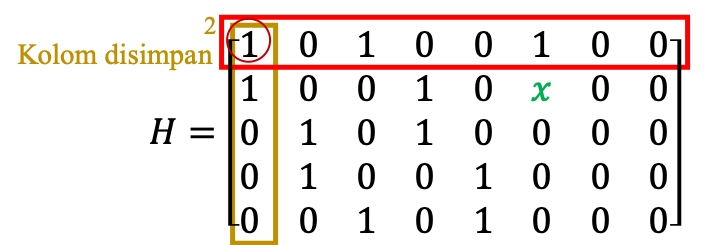
\includegraphics[scale=0.65]{gambarafa/step6}
		\centering 
	\end{figure}
	\begin{itemize}
		\item[5.] Iterasi ke-2 Algoritma \textit{Anti Girth}-4, menyimpan kolom dari elemen 1 yang ditemukan pada proses pengecekan di iterasi ke-1. 
		\item [6] Kemudian melakukan pengecekan akhir, yaitu apabila
		\begin{equation}
			H_{Baris\_simpan, Kolom\_simpan}=1,
		\end{equation}
		pada $x$ akan terbentuk \textit{girth} 4 jika $x$ berelemen 1, sehingga $x$ akan berpindah ke \textit{check node} dengan CND minimal berikutnya dan melakukan pengecekan lagi.
	\end{itemize}
	
	
	
	
	
\end{frame}
%=======================================================

%%--------------------------
%\begin{frame}{Encoding of LDPC Codes}
%%--------------------------
%\begin{columns}
%\column{.45\textwidth}
%\begin{figure}
%\centering
%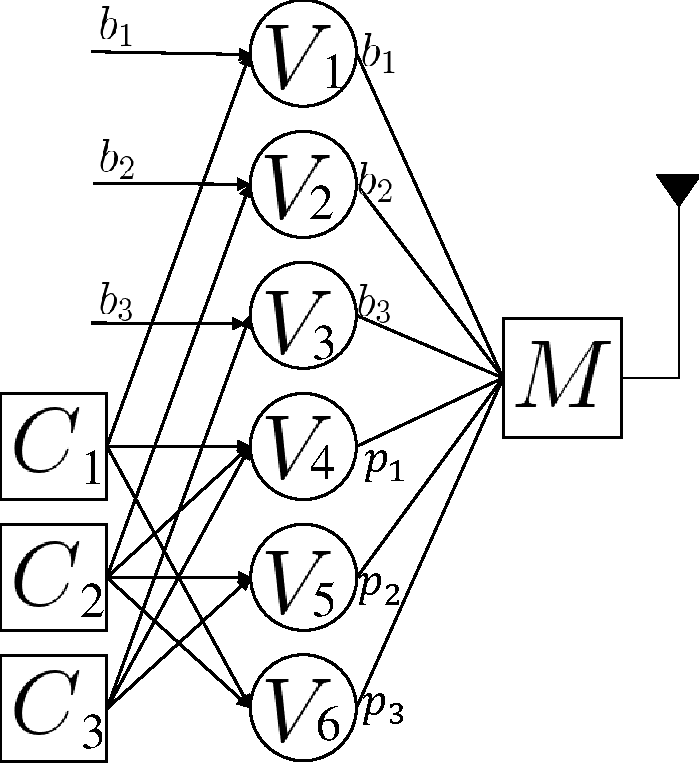
\includegraphics[scale=0.4]{pics/encoder2.pdf}
%\caption{Example for Tanner graph of Generator matrix LDPC codes.}
%\end{figure}
%
%\column{.55\textwidth}
%Information bits $b=\{b_1, b_2, ..., b_k\}$ are generated randomly, where $k$ is the number of bits in one block code.
%Generator Matrix $\mathbf{G}$ shows CND $ \mathbf{C} $, \textit{interleaver} $\Pi_x$, and VND $ \mathbf{V} $ in transmitter. The encoded codeword $\mathbf{c}$ can be written as
%\begin{equation}
% \mathbf{c}=\mathbf{b\:G}.
% \label{eqc}
%\end{equation}
%$c(k)$ is mapped to the complex modulation $M$ based on
%\begin{eqnarray}
%x(k)=\frac{1}{\sqrt{2}}[(1-2c(k))+j(1-2c(k))].
%\end{eqnarray}
%
%\end{columns}
%\end{frame}




%--------------------------
\begin{frame}{The LDPC Codes Constructed  Using PEG Algortihm}
%-------------------------- 

\begin{figure}
	\centering 
	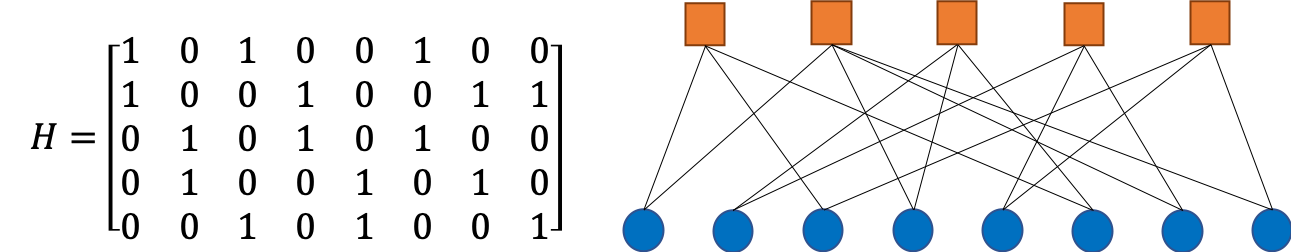
\includegraphics[scale=0.6]{gambarafa/PEGH}
	\centering 
	
	
\end{figure}
\begin{itemize}
	\item Matriks \textit{parity check} LDPC \textit{codes} $H$, dengan VND setiap kolomnya 2 yang dibentuk menggunakan PEG.  
	\item Matriks \textit{parity check} yang terbentuk tidak memiliki \textit{girth}-4.
\end{itemize}



\end{frame}
%=======================================================
\begin{frame}{Tree Graph of LDPC Codes}
	%-------------------------- 
	\vspace{-0.5cm}
	\begin{figure}
		\centering 
		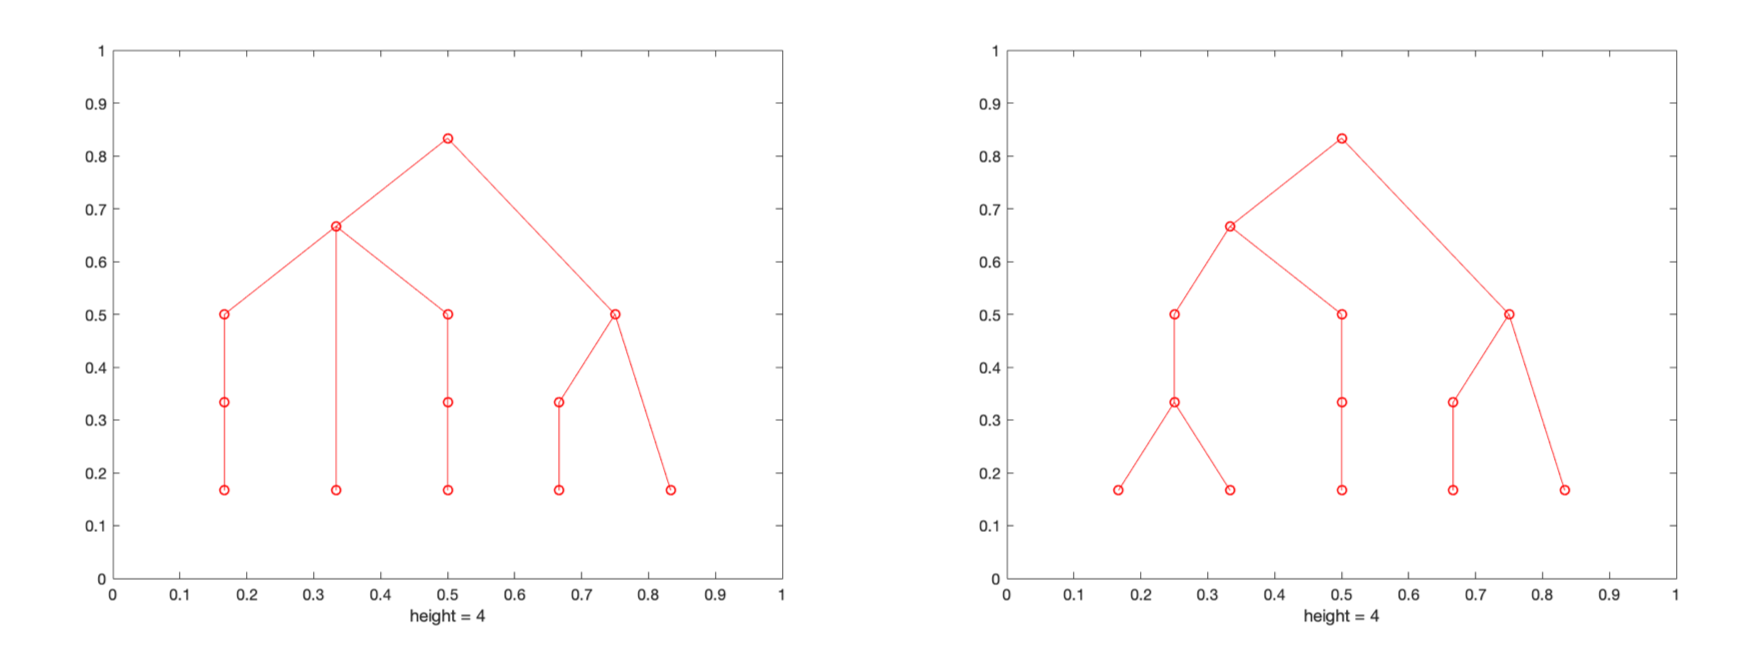
\includegraphics[scale=0.5]{gambarafa/treegrafmatlab2}
		\centering 
		
		
	\end{figure}
	\begin{itemize}
		\item Graf pohon matriks \textit{parity check random} LDPC \textit{codes} dan matriks \textit{parity check} LDPC \textit{codes} yang dirancang menggunakan PEG  pada \textit{variable node} ke-dua menggunakan MATLAB.
	\end{itemize}
	
	
	
\end{frame}
%=======================================================
\begin{frame}{Tree Graph of Random LDPC Codes}
	%-------------------------- 
	\vspace{-1.25cm}
	\begin{figure}
		\centering 
		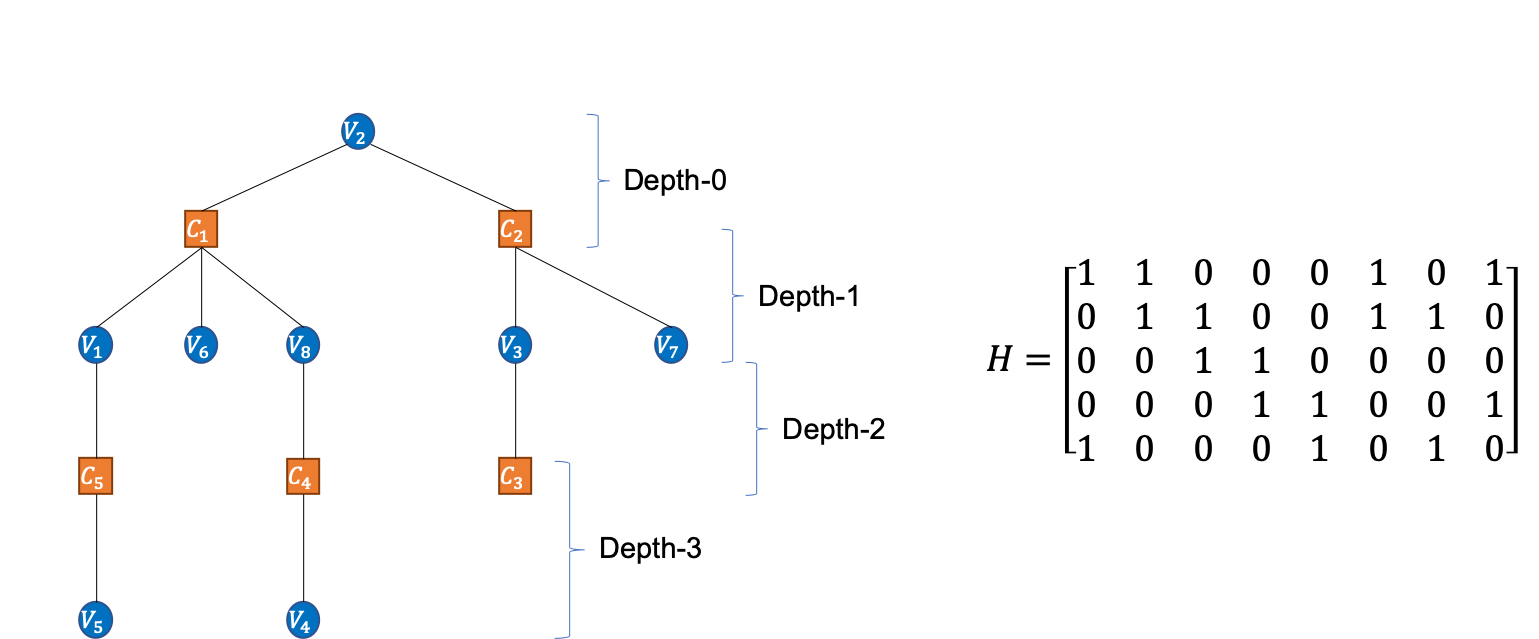
\includegraphics[scale=0.55]{gambarafa/kkk}
		\centering 
		
		
	\end{figure}
	\begin{itemize}
		\item Graf pohon dari matriks \textit{parity check random} LDPC \textit{codes} pada \textit{variable node} ke-dua memiliki nilai depth $l=3$. 
	\end{itemize}
	
	
	
	
\end{frame}


\begin{frame}{Tree Graph of LDPC Codes using PEG}
	%-------------------------- 
	\vspace{-0.5cm}
	\begin{figure}
		\centering 
		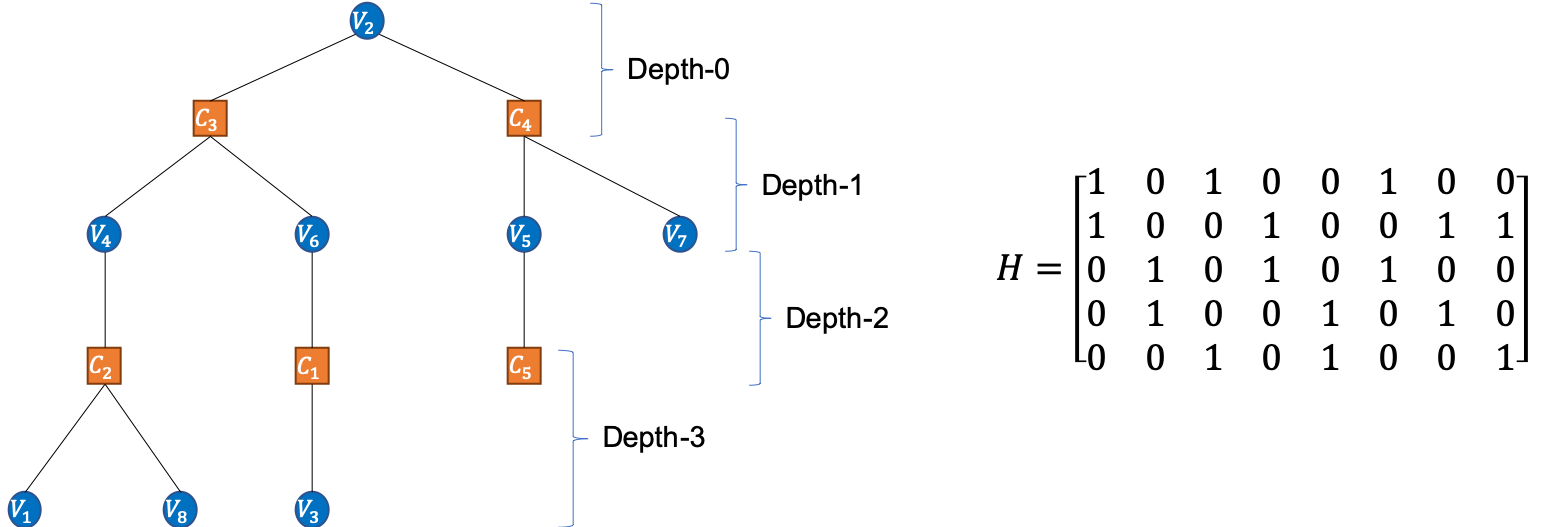
\includegraphics[scale=0.55]{gambarafa/withmatlabpeg}
		\centering 
		
		
	\end{figure}
	\begin{itemize}
		\item Graf pohon dari matriks \textit{parity check} LDPC \textit{codes} yang dirancang menggunakan PEG pada \textit{variable node} ke-dua memiliki nilai depth $l=3$. 
	\end{itemize}
	
	
	
	
\end{frame}

\begin{frame}{Proposed Girth Calculation Method}
	%-------------------------- 
	

	\begin{columns}
		\column{.5\textwidth}
	\vspace{-2cm}
	\begin{figure}
		\centering 
		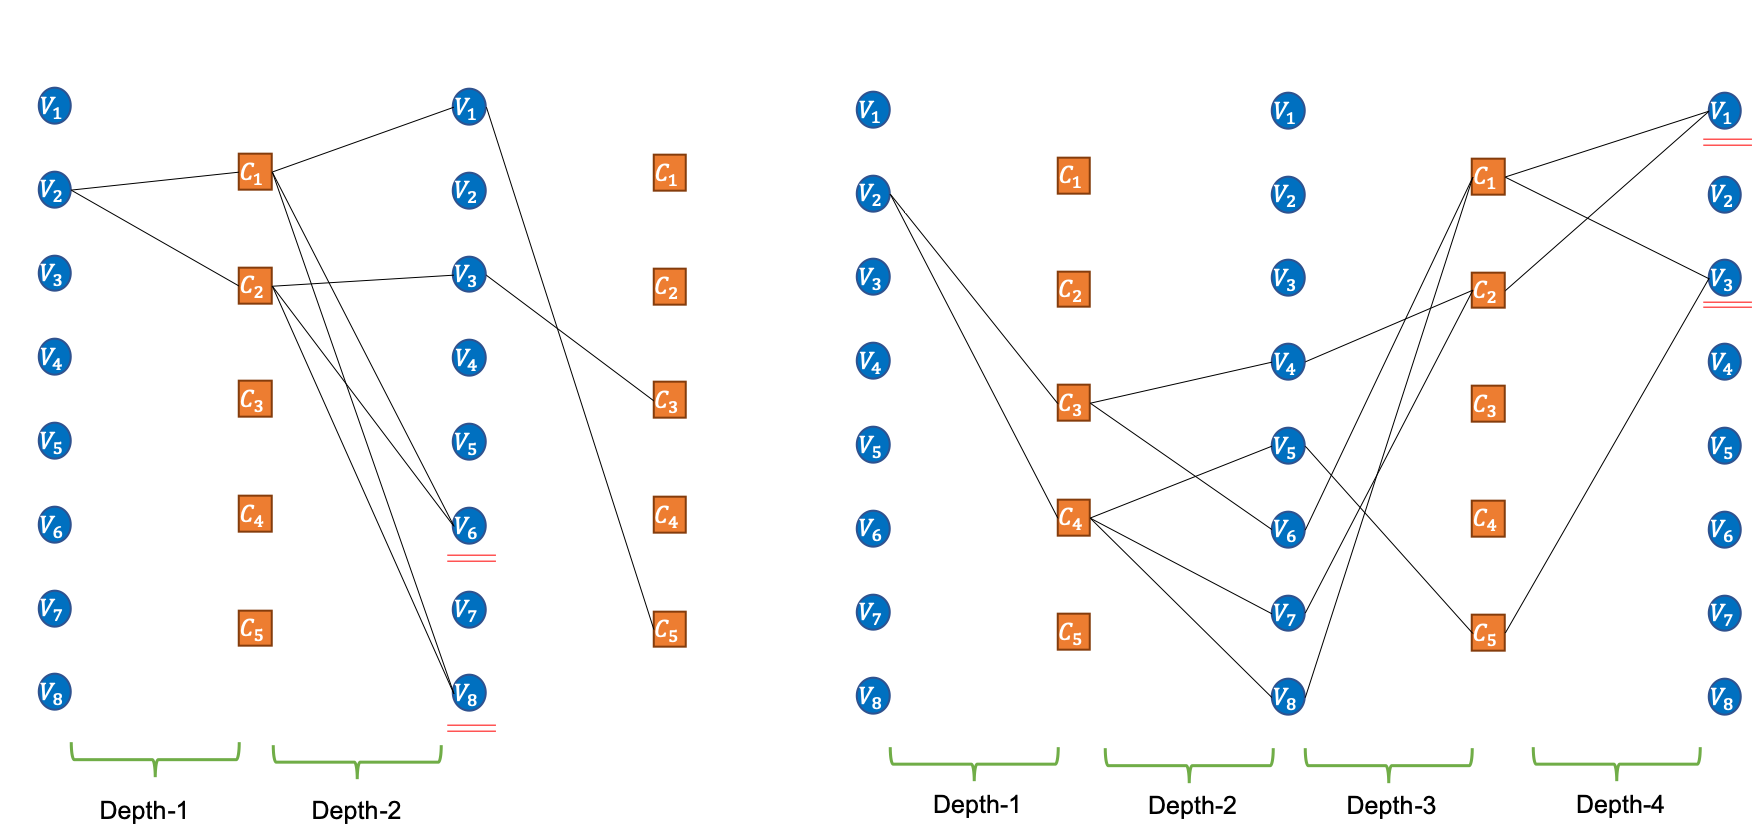
\includegraphics[scale=0.25]{gambarafa/hitunggirth}
		\centering 
	\end{figure}
		\column{.5\textwidth}
		\textit{Local girth} dapat dihitung dengan menggunakan teknik pembuatan graf pohon PEG yang dimodifikasi. Berikut langkahnya:
		\begin{enumerate}
			\item Tentukan satu \textit{variable node} dan sebarkan \textit{edges}-nya sesuai dari matriks.
			\item Sebarkan \textit{edges} terus menerus sampai terdapat \textit{node} yang tidak dapat menyebarkan \textit{edge}.
			\item Hitung \textit{branch} $b$ dimulai dari satu, lalu dengan menggunakan persamaan
			\begin{equation}
			g=b\times 2,
			\end{equation}
			maka nilai \textit{local girth} dapat diketahui.
		\end{enumerate}
	\end{columns}
	
	
\end{frame}


\begin{frame}{Girth Distributions}
%$R=\frac{11}{15}$
%\begin{eqnarray}
%\lambda (x)&=&\frac{1}{270}x+\frac{71}{270}x^{2}+\frac{192}{270}x^{3}+\frac{6}{270}x^{12},\\
%\rho(x)&=&\frac{7}{48}x^{15}+\frac{17}{48}x^{16}+\frac{18}{48}x^{17}+\frac{6}{48}x^{18},
%\end{eqnarray}
%$R=\frac{7}{9}$
%\begin{eqnarray}
%\lambda (x)&=&\frac{1}{270}x+\frac{71}{270}x^2+\frac{198}{270}x^3,\\
%\rho(x)&=&\frac{7}{60}x^{11}+\frac{29}{60}x^{12}+\frac{24}{60}x^{13},
%\end{eqnarray}
%$R=\frac{37}{45}$
%\begin{eqnarray}
%\lambda (x)&=&\frac{1}{270}x+\frac{71}{270}x^{2}+\frac{192}{270}x^{3}+\frac{6}{270}x^{12},\\
%\rho(x)&=&\frac{7}{72}x^{9}+\frac{11}{72}x^{10}+\frac{36}{72}x^{11}+\frac{12}{72}x^{12} \nonumber \\ &&+\frac{6}{72}x^{13}.
%\end{eqnarray}

	\begin{figure}
	\centering 
	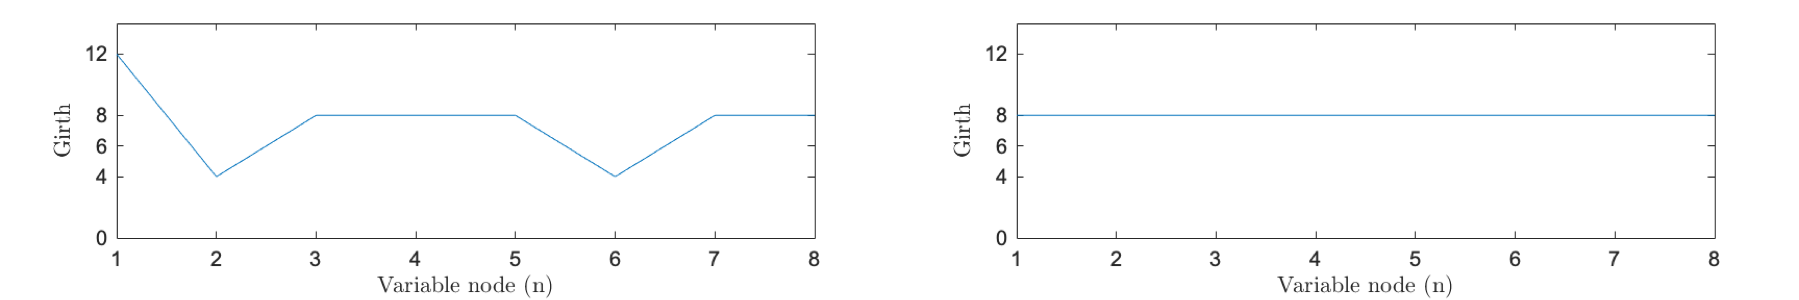
\includegraphics[scale=0.45]{gambarafa/girthdisemua}
	\centering 
	
	
\end{figure}
\begin{itemize}
	\item Hasil penghitungan \textit{girth} dari matriks \textit{parity check random} LDPC \textit{codes} dan LDPC \textit{codes} yang dirancang menggunakan algoritma PEG dengan nilai VND yang sama. 
\end{itemize}

\end{frame}

%\begin{frame}{Extrinsic Information Transfer (EXIT) Chart}
%\begin{columns}
%\column{0.7\textwidth}
%\begin{itemize}
%%\item Tujuan digunakan EXIT \textit{chart} pada jaringan super padat adalah mendesain jaringan \textit{Internet-of-Things} (IoT) di suatu kota. 
%\item EXIT chart use mutual information $I=1-v$ where $v$ is erasure probability $v=\{p,q\}$.
%\item Parameter $p$ and $q$ is erasure probability for CND and VND.
%\item EXIT chart shows extrinsic mutual information from VND
%\begin{eqnarray}
%I_{E,VND}(x)&=&1-\lambda(p) \nonumber\\
% &=&1-\lambda(1-I_{A,VND}), 
%\end{eqnarray}
%and extrinsic mutual information from CND
%\begin{eqnarray}
%I_{E,CND}(x)&=&\omega(1-q) \nonumber\\
% &=&\omega(I_{A,CND}).
%\end{eqnarray}
%\end{itemize}
%\column{0.35\textwidth}
%\begin{figure}
%	\centering
%	\includegraphics[width=0.8\textwidth]
%		{pics/erasure.pdf}
%		\caption{Edge probability from CND and VND}
%\end{figure}
%\end{columns}
%\end{frame}
     

%============================================================================
%==========================================================================
\section{Performance Evaluations}
%\begin{frame}
%\tableofcontents[currentsection,currentsubsection]
%\end{frame}
%--------------------------
%\begin{frame}{Performance Evaluation (1): EXIT Analysis}
%%--------------------------
%\begin{columns}
%\column{.5\textwidth}
%\vspace{-30pt}
%%\begin{figure}
%%\centering 
%%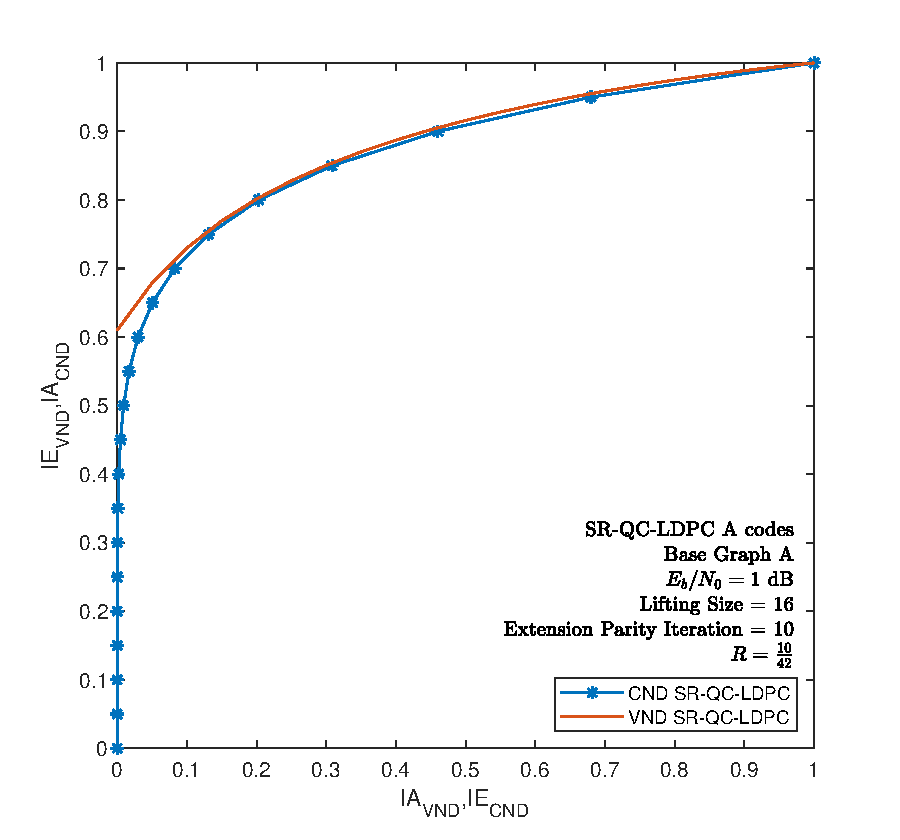
\includegraphics[scale=0.4]{pics/EXIT_QC_1.pdf}
%%\caption{EXIT chart of the proposed SR-QC-LDPC-A codes.}
%%\label{coba1} %~\ref{kucing}
%%\end{figure}
%
%\column{.5\textwidth}
%\vspace{-30pt}
%%\begin{figure}
%%\centering 
%%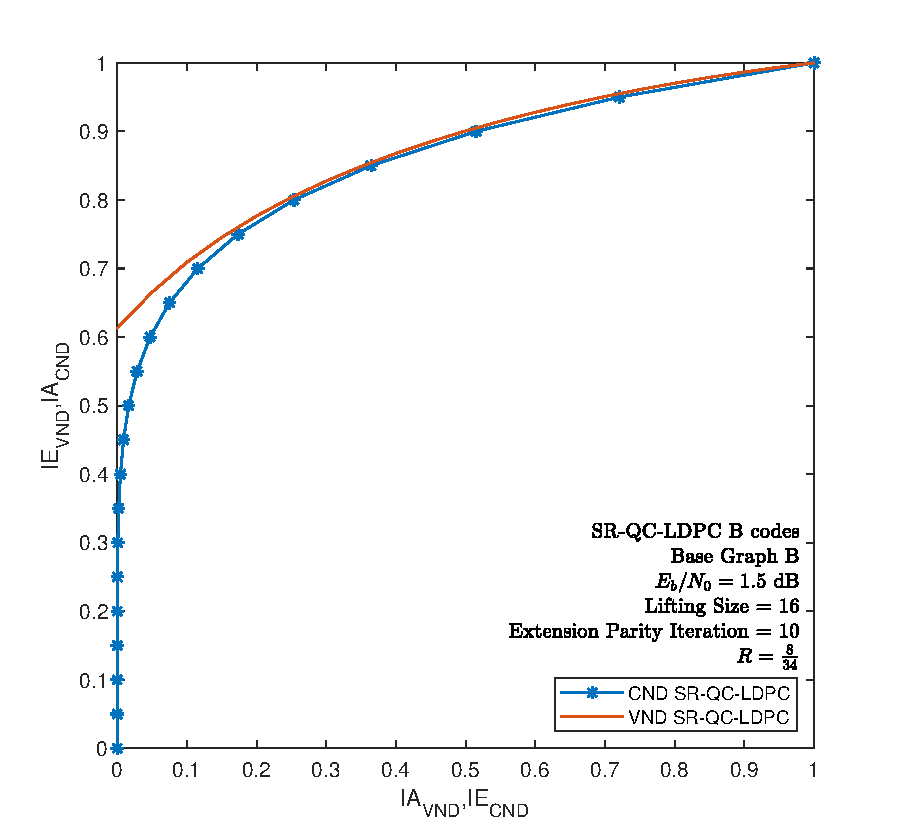
\includegraphics[scale=0.4]{pics/EXIT_QC_3.pdf}
%%\caption{EXIT chart of the proposed SR-QC-LDPC-B codes.}
%%\label{coba2} %~\ref{kucing}
%%\end{figure}
%\end{columns}
%EXIT curve of VND and CND shows that gap is minimal expressing that the loss of the proposed SR-QC-LDPC codes is minimal.
%\end{frame}

%--------------------------
\begin{frame}{Performance Evaluation on AWGN Channel}
%--------------------------
\vspace{-25pt}
\begin{columns}
\column{.5\textwidth}
\begin{figure}
\centering 
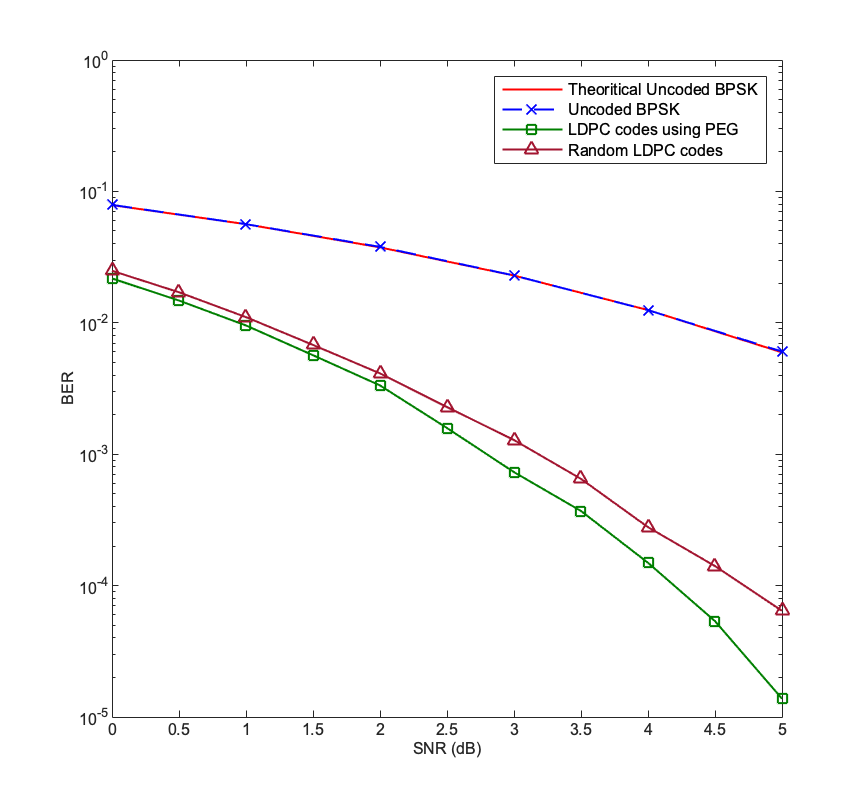
\includegraphics[scale=0.5]{gambarafa/sem}
%\caption{BER performances of DVB-T2 LDPC codes with $R=\frac{4}{9}$ under AWGN channel.}
\label{awgn} %~\ref{kucing}
\end{figure}
\column{.5\textwidth}
\begin{itemize}
\item Simulasi menggunakan iterasi pada LDPC \textit{codes} sebanyak $t=80$ dan menggunakan modulasi BPSK.
\item LDPC \textit{codes} yang dirancang menggunakan PEG memiliki kinerja yang lebih baik dibandingkan \textit{random} LDPC \textit{codes}  dengan ukuran matriks dan VND yang sama.
%\item The proposed SR-QC-LDPC codes is comparable with 5G NR QC-LDPC codes, where the obtained gap is about 0.75--1~dB.
\end{itemize}
\end{columns}
\end{frame}

%--------------------------
%\begin{frame}{Performance Evaluation using EXIT chart}
%%--------------------------
%\begin{columns}
%
%\column{.45\textwidth}
%\vspace{-25pt}
%\begin{figure}
%\centering 
%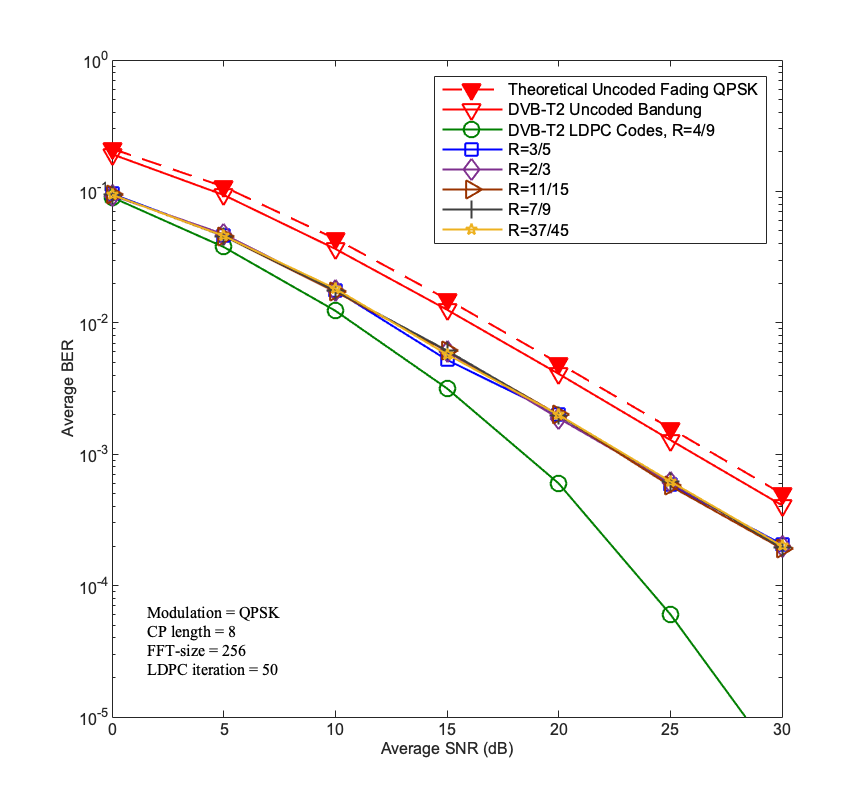
\includegraphics[scale=0.4]{gambarafa/coded-2}
%\caption{BER performances Downscaled DVB-T2 LDPC codes codes under Bandung Channel models.}
%\label{fading} %~\ref{kucing}
%\end{figure}
%\column{.55\textwidth}
%\begin{itemize}
%
%\justifying
%\item The BER Performances of DVB-T2 LDPC codes with $R~=~\left \{ \frac{4}{9}, \frac{3}{5}, \frac{2}{3},\frac{11}{15},\frac{7}{9},\frac{37}{45} \right \}$ are evaluate under Bandung Channel models\footnotemark[1].
%\item The best performances of Downscaled LDPC codes DVB-T2 on is achieved $10^{-4}$ at $R=\frac{4}{9}.$
%
%\end{itemize}
%\end{columns}
%\blfootnote{\tiny{D. Fitriyani, K. Anwar, and D. M. Saputri, "Study on Radio Frequency Profile of Indonesia Digital Television DVB-T2 for Urban Areas", in 2019.}}
%
%\end{frame}


%==============================================================================
%==============================================================================




%============================================================================
%==========================================================================

\section{Conclusion}
%\begin{frame}
%\tableofcontents[currentsection,currentsubsection]
%\end{frame}
\begin{frame}{Conclusion}
%--------------------------
\begin{itemize}
\justifying
\item Telah melakukan perancangan matriks \textit{parity} \textit{check} LDPC \textit{codes}  dengan menggunakan algoritma PEG yang digabungkan dengan algoritma Anti \textit{Girth}-4 . 
\item Mengusulkan sebuah algoritma untuk menghindari \textit{girth}-4 pada matriks \textit{parity} \textit{check} LDPC \textit{codes} dan teknik untuk menghitung \textit{girth} dari \textit{matriks parity check} LDPC \textit{codes}.
%\item The gap between DVB-T2 LDPC codes  $N_{LDPC}=16200$ and downscaled DVB-T2 LDPC codes $N_{LDPC}=270$ is about $2.8~dB$.
\item Algoritma PEG  memudahkan dalam memodifikasi dan merancang LDPC \textit{codes} yang memiliki nilai \textit{girth} besar.
%\item The best code rate of downscaled DVB-T2 LDPC codes under Bandung Channel model is $R=\frac{4}{9}$.
\item Metode kedua dari PEG pada LDPC codes akan cenderung menyamakan CND dari matriks parity \textit{check codes} yang terbentuk. 
%\item The performances of rateless capability have also been confirmed to be better than that of the fixed rate under the fading channels. 
%\item The codes are expected to be useful for further development of dynamic channel changes.
\end{itemize}
\end{frame}



%--------------------------
%\begin{frame}{Conclusion}
%%--------------------------
%\begin{itemize}
%\justifying
%\item This paper has proposed SR-QC-LDPC codes inspired from the Raptor encoding principle of 5G NR QC-LDPC codes. 
%\item The SR-QC-LDPC codes have been designed by reducing the matrix size and removing the high degree, of which the final designs are evaluated using EXIT chart. 
%\item We found that the codes have excellent EXIT curve matching where small gap is kept although the size of the matrix is reduced. 
%\item The performances of rateless capability have also been confirmed to be better than that of the fixed rate under the fading channels. 
%\item The codes are expected to be useful for further development of dynamic channel changes.
%\end{itemize}
%\end{frame}

%==============================================================================
%==============================================================================

\end{document}
